\documentclass[12pt, a4paper]{article}
\usepackage{enumerate}
\usepackage{amsmath}
\usepackage{amssymb}
\usepackage{blkarray}
\usepackage{geometry}
\usepackage{float}
\usepackage{graphicx}
\usepackage[linesnumbered, ruled]{algorithm2e}
\usepackage{forest}
\usepackage{diagbox}
\usepackage{cite}
\usepackage{url}
\usepackage{subfig}

\geometry{left = 2.0cm, right = 2.0cm}

\SetKwInOut{Input}{Input}
\SetKwInOut{Output}{Output}
\SetKwProg{Fn}{Function}{:}{end}
\SetKwFunction{RS}{equalProb}
\SetKwFunction{TS}{TriangleSum}
\SetKwFunction{main}{main}

\title{
    \begin{figure}[H]
        \centering
        
\includegraphics[width=7cm, height=5cm]{AAA.png}
    \end{figure}
    VE477 Introduction to Algorithms\\ 
    Homework 4}
\author{Taoyue Xia, 518370910087}
\date{2021/10/26}

\begin{document}
\maketitle

\newpage

\section*{Ex. 1 --- Time vs. space}
\begin{enumerate}
    \item For $2^{64}$ operations:
          $$t = \frac{2^{64}}{33.86\cdot 10^{15}} = 544.79\, s$$
          For $2^{80}$ operations:
          $$t = \frac{2^{80}}{33.86\cdot 10^{15}} = 35703656.81s = 413.23\ days$$
    \item First calculate how much time one computer need to perform $2^{64}$ operations:
          $$t = \frac{2^{64}}{4\cdot 3.8\cdot 10^9} = 1213601583.79\, s$$
          Then divide time with total seconds in one day, which is 86400, we can get the number of computers needed:'
          $$n = \frac{t}{86400} = 14046.31$$
          Which means that we need 14047 computers with Intel Core i7-5775R CPU to perform $2^{64}$ operations in one day.

          For $2^{80}$ operations, using the same method of calculation:
          $$t = \frac{2^{80}}{4\cdot 3.8\cdot 10^9} = 79534593395699.28\, s$$
          $$n = \frac{t}{86400\cdot 30} = 30684642.51$$
          Which means that we need 30684643 computers with Intel Core i7-5775R CPU to perform $2^{80}$ operations in one month.
    \item $$2^{64}\, bits = 2^{61}\, Bytes = 2^{51}\, KB = 2^{41}\, MB = 2^{31}\, GB = 2^{21}\, TB$$
          Then the number of hard disks needed is:
          $$n = \frac{2^{21}}{16} = 2^{17}$$
          Which means that we need $2^{17}$ hard disks to store $2^{64}$ bits data.

          For $2^{80}$ bits data, calculate as above:
          $$2^{80}\, bits = 2^{77}\, Bytes = 2^{67}\, KB = 2^{57}\, MB = 2^{47}\, GB = 2^{37}\, TB$$
          $$n = \frac{2^{37}}{16} = 2^{33}$$
          Which means that we need $2^{33}$ hard disks to store $2^{80}$ bits data.
\end{enumerate}

\section*{Ex. 2 --- Critical thinking}
We can use an algorithm known as ``Reservoir Sampling'' to handle this problem, the algorithm is like:

\begin{algorithm}[!htb]
    \caption{Reservoir Sampling}
    \Input{A Set $S$ of $n$ integers, a number $k$}
    \Output{A set $S^\prime$ of $k$ elements with equal probability to be chosen}

    \Fn{\RS{$S$, $k$}}{
        $S^\prime \leftarrow$ an empty set\;
        \For{$i = 0$ to $k-1$}{
            $S^\prime [i] = S[i]$\;
        }

        \For{$i = k$ to $n-1$}{
            $j \leftarrow$ a random integer ranging from $0$ to $i-1$\;
            \If{$j < k$}{
                $S^\prime [j] \leftarrow S[i]$\;
            }
        }
        \KwRet{$S^\prime$}\;
    }
\end{algorithm}

\textbf{Proof of equal probability}:

Let's prove it by induction
\begin{itemize}
    \item When $n = 1$, it is obvious that the probability of selection is $1/1 = 1$.
    \item Suppose that for choosing a subset of $k$ integers, $n$ integers are chosen with equal probability $\frac{k}{n}$ in a set. 
          Then we know that the $n+1_{th}$ integer will replace one of the $k$ integers with probability $P_1 = \frac{k}{n+1}$. 
          So the probability of not replacing is $1 - P_1$. 

          Then if the $n+1_{th}$ integer is chosen to replace, but is not the one we expected, the probability will be:
          $$P_2 = \frac{k}{n+1} \cdot (1 - \frac{1}{k}) = \frac{k-1}{k}P_1$$
          So the probability for one integer in the $k$-integer set to stay is $P_3 = 1 - P_1 + P_2 = \frac{n}{n+1}$.
          Since in the previous $n$-integer case, each is selected with probability $\frac{k}{n}$, therefore, 
          when added an $n+1_{th}$ integer, all the integers should have the probability of $P_3\cdot \frac{k}{n} = \frac{k}{n+1}$ to be selected. 

          Proof done.
\end{itemize}

\section*{Ex. 3 --- Algorithm and complexity}
\begin{enumerate}
    \item The pseudocode is like:

          \begin{algorithm}[!htb]
              \caption{Triangle sum of one line}
              \Input{an integer $i$}
              \Output{The sum of the $i_{th}$ line}

              \Fn{\TS{$i$}}{
                  \If{$i = 1$}{
                      \KwRet{$[1]$}\;
                  }
                  $S \leftarrow$ \TS{$i - 1$}\;
                  length $\leftarrow$ $S$.length\;

                  $SS \leftarrow$ and empty set with preallocation of $2i-1$ slots\;
                  \For{$j=0$ to $i-1$}{
                      \uIf{$j=0$}{
                          $SS[0],\ SS[2i-2] \leftarrow 1$\;
                      }
                      \uElseIf{$j=1$}{
                          \uIf{length = 1}{
                            $SS[1],\ SS[2i-3] \leftarrow 1$\;
                          }
                          \Else{
                              $SS[1],\ SS[2i-3] \leftarrow S[0] + S[1]$\;
                          }
                      }
                      \Else{
                          $SS[j], SS[2i-2-j] \leftarrow S[j-2] + S[j-1] + S[j]$\;
                      }
                  }
                  \KwRet{SS}\;
              }

              \Fn{\main{$i$}}{
                  $S \leftarrow$ \TS{$i$}\;
                  sum $\leftarrow$ sum($S$)\;
                  \KwRet{sum}\;
              }
          \end{algorithm}
    \item Given integer $i$, The time complexity is $\mathcal{O}(i^2)$.
          
          To get the sum of the $i_{th}$ line, we just need to loop for $1 + 2 + 3 + \dots + i - 1 = \frac{n(n-1)}{2}$ times, 
          and with recursion, we can get the final answer. Therefore, the time complexity is $\mathcal{O}(n^2)$.

\end{enumerate}

\section*{Ex. 4 --- From SAT to 3-SAT}
\begin{align*}
    &\quad\ \, (x_1\vee x_2\vee \lnot x_3\vee x_4\vee x_5\vee \lnot x_6) \wedge (\lnot x_1\vee \lnot x_2\vee x_3\vee \lnot x_4\vee x_5\vee x_6)\\
    &\quad\ \, \wedge (x_1\vee \lnot x_2\vee \lnot x_3\vee x_4\vee x_5\vee \lnot x_6) \wedge (x_1\vee \lnot x_2)\\
    &= (x_1\vee x_2\vee u_3) \wedge (\lnot u_3\vee \lnot x_3\vee u_4) \wedge (\lnot u_4\vee x_4\vee u_5) \wedge (\lnot u_5\vee x_5\vee \lnot x_6)\\
    &\quad\ \, \wedge (\lnot x_1\vee \lnot x_2\vee u_3^\prime) \wedge (\lnot u_3^\prime \vee x_3\vee u_4^\prime) \wedge (\lnot u_4^\prime \vee \lnot x_4\vee u_5^\prime) \wedge (\lnot u_5^\prime \vee x_5\vee x_6)\\
    &\quad\ \, \wedge (x_1\vee \lnot x_2\vee u_3^\circ) \wedge (\lnot u_3^\circ \vee \lnot x_3\vee u_4^\circ) \wedge (\lnot u_4^\circ \vee x_4\vee u_5^\circ) \wedge (\lnot u_5^\circ \vee x_5\vee \lnot x_6)\\
    &\quad\ \, \wedge (x_1\vee \lnot x_2\vee u_1) \wedge (x_1\vee \lnot x_2\vee \lnot u_1)
\end{align*}

\section*{Ex. 5 --- Clique problem}
\begin{enumerate}
    \item The Clique problem aims to find a complete subgraph of a graph, in which all vertices are adjacent to each other.
    \item \textbf{Certificate}: A subgraph $S$ of the original graph $G$ as a clique.
          
          \textbf{Verification}: If we aim to find a $k$-clique, which is the subgraph of $G$ with exact $k$ vertices connected to each other. 
          Then we can check if $S$ satisfies the requirement. Firstly, checking whether $S$ contains exactly $k$ vertices takes $\mathcal{O}(1)$ time. 
          Then, checking whether each vertex is connected to each other takes $\mathcal{O}(k^2)$ time, 
          since we just need to check if each vertex is on one end of $k-1$ edges, which takes $1+2+\dots+k-1 = \frac{k(k-1)}{2}$ times of check. 
          Therefore, the verification process takes polynomial time.

          From the above, we can say that Clique problem is in $\mathcal{NP}$.
    \item Firstly, make some definitions:
          
          Let $C_1, C_2, \dots, C_k$ be the $k$ clauses.\\
          Let $x_{i,1}, x_{i,2}, x_{i,3}$ be the three literals of $C_i$, $i\in \{1,2,\dots,k\}$.\\
          Then we make every $x_{i,j}$ to be a vertex in $G$, and no edge exists between vertices from the same clause, 
          and between two literals which are negation of each other.

          \begin{itemize}
              \item[$\Rightarrow$] If $F$ is satisfiable, we can choose one vertex from each clause, which satisfies the above requirement. 
                                   Since if each two of them doesn't belong to the same clause or are negation of each other, 
                                   there will be an edge between, assign them to be true, thus we can find a $k$-clique in $G$.
              \item[$\Leftarrow$] If $G$ has a $k$-clique, then each vertex comes from a distinct clause and no two are negations of each other. 
                                  Then, if we assign each literal which represents the vertex to be true, we can prove that $F$ is satisfiable. 
          \end{itemize}
          Therefore, $F$ is satisfiable if and only if $G$ has a $k$-clique.

          \begin{figure}[!htb]
              \centering
              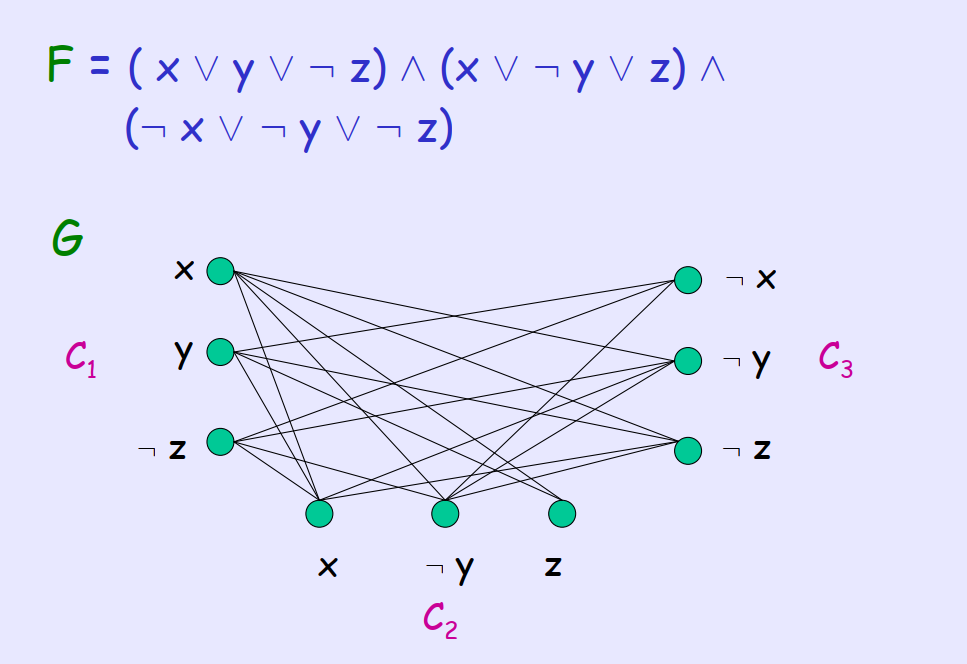
\includegraphics[width=10cm, height=6.5cm]{h4.png}
              \caption{An example of construction}
          \end{figure}
    \item From the above question, we proved that we can construct an easy transformation (polynomial time) from 3-SAT to the Clique problem. 
          Since 3-SAT is $\mathcal{NP}$-complete, we can reduce 3-SAT to Clique problem. Therefore, the Clique problem is $\mathcal{NP}$-complete.
\end{enumerate}

\section*{Ex. 6 --- IND-SET problem}
\begin{enumerate}
    \item The maximum independent set problem aims to find the largest independent set of a graph, 
          and an independent set is a subset of a graph with size $k$ in which no two vertices are adjacent to each other.
    \item The IND-SET decision problem aims to determine an independent set of an undirected graph.
    \item \textbf{Certificate}: A subset $S$ of Graph $G$ with size $k$.
          \textbf{Verification}: Firstly, checking whether the set has $k$ vertices takes $\mathcal{O}(1)$ time. 
          Then, checking that no two vertices are adjacent to each other takes $\mathcal{O}(k)$ time. 
          According to the above, we can verify the correctness in polynomial time. Therefore, IND-SET is in $\mathcal{NP}$.
    \item We can simply create a new Graph $G^\prime$ which is a complement of original graph $G$, 
          which means that for all edges in $G$, they don't exist in $G^\prime$. In this sense, if $G$ has a $k$-clique, 
          then in $G^\prime$, those $k$ vertices will not be adjacent to each other, 
          which means that $G^\prime$ has an independent set of size $k$, and vice versa.\\
          Therefore, ``$G$ has a $k$-clique'' is equivalent to ``$G^\prime$ has an independent set of size $k$''.
    \item In the above question, we have proved that Clique problem can be reduced in polynomial time to IND-SET problem. 
          Therefore, the IND-SET problem is $\mathcal{NP}$-complete.
\end{enumerate}


\end{document}